\section{Durchführung}
\label{sec:Durchführung}

\subsection{Untersuchung eines Acrylblocks mit dem A-Scan}

Zunächst werden die Abmessungen des Acrylblocks (siehe Abb. \ref{fig:Block}) notiert.
Eine 2 MHz Sonde wird mit bidestiliertem Wasser an den Block gekoppelt.
Mit dem Impuls-Echo-Verfahren wird von beiden Seiten die Schalllaufzeit gemessen,
um sowohl die Größe als auch die Lage der Bohrungen zu bestimmen.
\begin{figure}
  \centering
  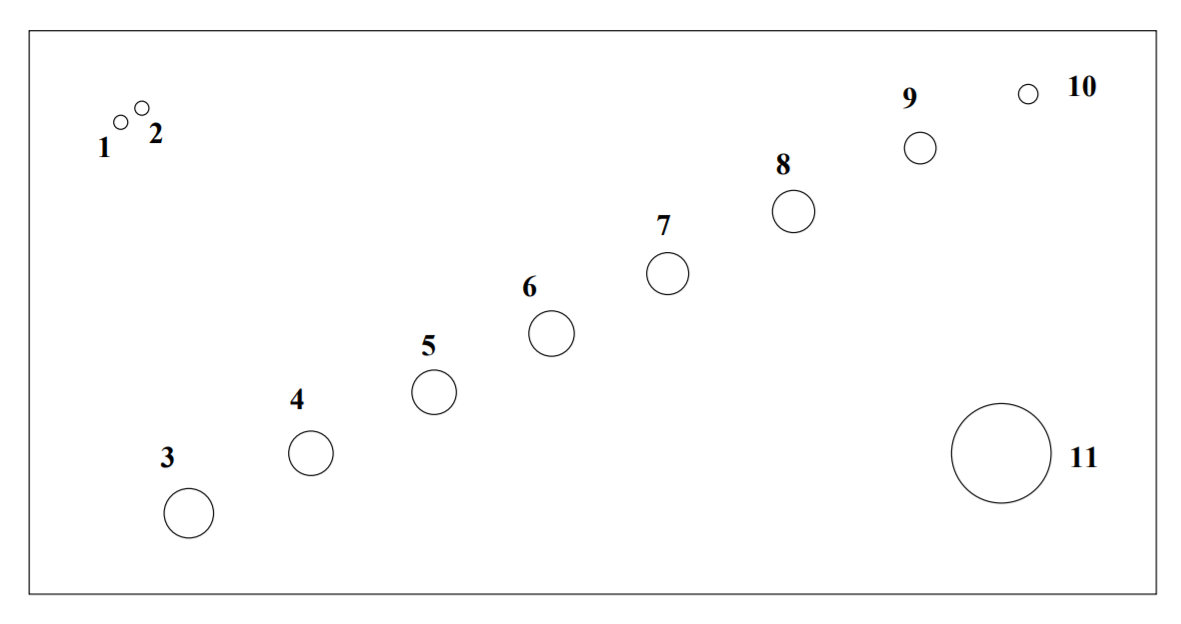
\includegraphics[height=5cm]{data/Block.png}
  \caption{Schematische Zeichnung des Acrylblocks. \cite{US2}}
  \label{fig:Block}
\end{figure}

\subsection{Untersuchung des Auflösungsvermögen}

Zwei benachbarte und kleine Bohrungen werden mit dem A Scan und einer 1,2 und 4 MHz Sonde untersucht werden.
Das Auflösungsvermögen der verschiedenen Sonden soll beurteilt werden.

\subsection{Untersuchung eines Acrylblocks mit dem B-Scan}

Eine 2 MHz Sonde wird auf der Längsseite auf den Block gekoppelt.
Zur Aufnahme eines B Scans wird die Sonde langsam und mit konstanter Geschwindigkeit über den Block geführt.
Auf der gegenüberliegenden Seite wird ebenfalls ein B Scan durchgeführt.

\subsection{Untersuchung eines Herzmodells mit dem TM-Scan}

Das Herzmodell besteht aus einem Doppelgefäß, das zu einem Drittel mit Wasser befüllt ist,
und einer beweglichen Membran, die periodisch gewölbt werden kann.
Mit Hilfe eines A Scan wird das enddiastolische Volumen (EDV) und das endsystolische Volumen (ESV) bestimmt.
Die Herzfrequenz wird mit einem TM Scan gemessen.
Aus diesen Größen wird abschließend das Herzvolumen bestimmt.
